%Now that the kernel is copied, we should remove all the dependencies that refers to classes not copied in the Hazel SystemDictionary. Even if it's easy to notice which dependencies are wrong, the way to automatically fix them is not that simple. The best way should be to dynamically create a NullPattern class and if a method points to a wrong class, just make it invoke the NullPattern's method instead. It means that you will double the number of classes, and it's not obvious to automatically build a NullPattern class. I've decided to simply removed the method and to flag them. This way I can know which methods have been removed, and analyze if the dependence make sense or not. 
%
%To help me in the analyze, I've write some tools to evaluate the impact of the addition of a collection of classes in the kernel. When the dependence is really bad, I used to open a report on the developers platform.
%
%I had the same kind of issues about class variables, and I've decided to set such variable at \ct{nil}.
%
%The problem with those methods is that at the end, the image can not be able to work. But due to the fact that only few people will using this tool, and that those people are aware of how the system is, and how the dependencies are, I think it is not a real problem, and moreover, this issues can be solved only by restructured the whole system to avoid dependencies as much as possible.
%
%During my analyzes, I have noticed that a lot of dependencies, especially from the Kernel package, should be removed and I have fixed a lot of them, to reduce the number of dependencies in Hazel, but in \gls{\gls{Pharo}} too.
%
%So at the end of this step, I have an isolated kernel with no more references to classes I haven't choose at the beginning, but still in the \gls{\gls{Pharo}} world (see Figure~\ref{KernelIsolation}).
%
%\begin{figure}[ht]
%	\centering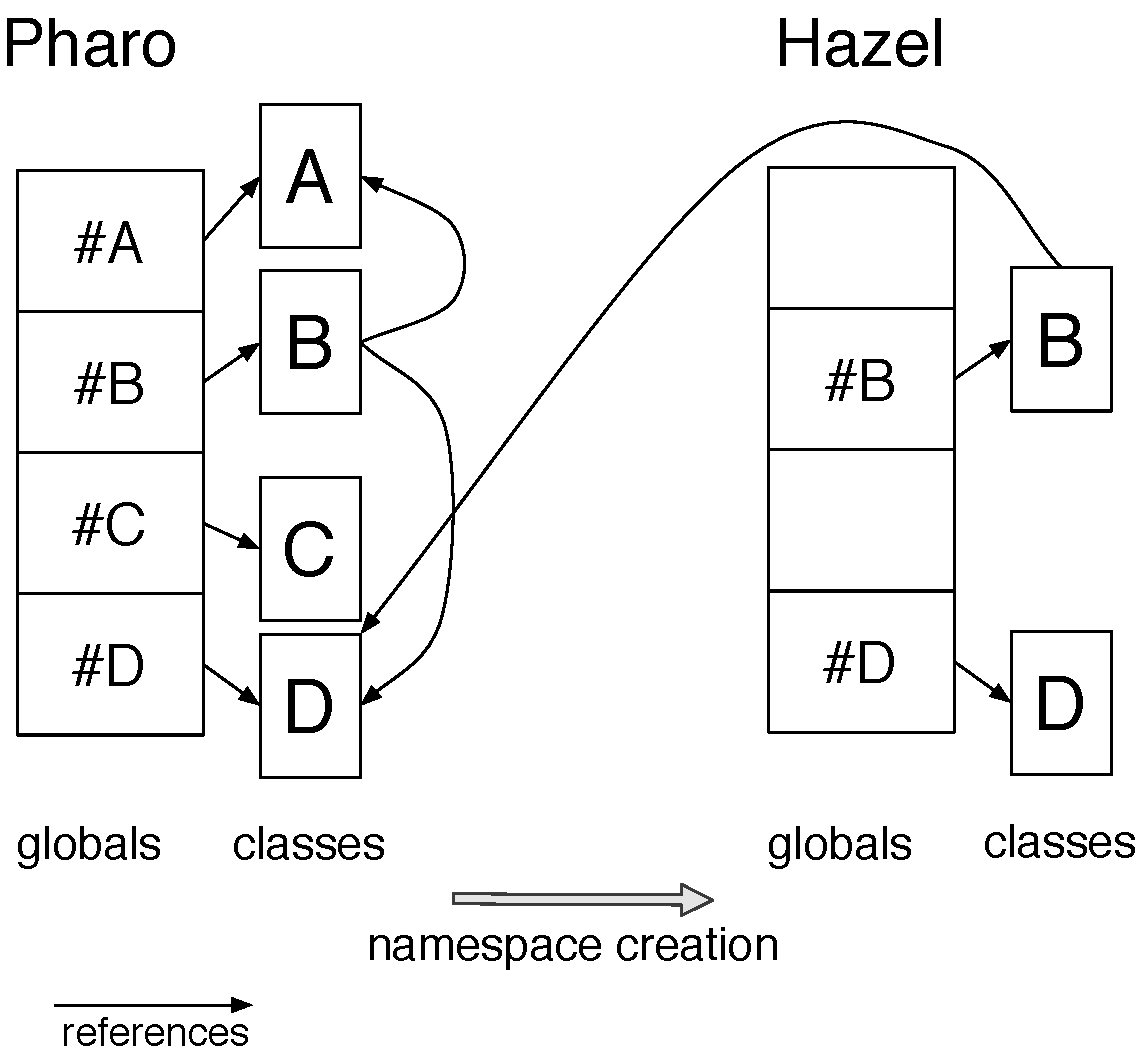
\includegraphics[height = 10cm]{figures/CleaningUnnecessaryRef}
%	\caption{Kernel Isolation}
%	\label{KernelIsolation}
%\end{figure}
%
%
%%% ------------------------------------------------------------ %%
%%
%%	From here I start trying no to use I anymore ^^
%%
%%% ------------------------------------------------------------ %%
%
%Now the Hazel SystemDictionary need to be fixed in order to only have methods depending on itself. To do that, all the methods from all the classes from Hazel SystemDictionary are browsed in order to fix their literals. At this step, we are sure that all the classes needed have already been copied. The problem is that in literals, their also references to global variables, class variables and pool variables, so we just have to check the case which is easy now \gls{TextConstants} (see section~\ref{TextConstants} page~\pageref{TextConstants}) is well restructured.
%
%In fact, those two steps (the copy and the fix) are done in only one pass to gain performance.
%
%Finally, some \glspl{primitive}\footnote{Especially \ct{becomeForward:} and \ct{primitiveChangeClassTo:}} were used to change the structure of the SystemDictionary to have it build with Hazel objects.
%
%Now all references are fixed, so Hazel SystemDictionary is now isolated from the \gls{\gls{Pharo}} world (see Figure~\ref{KernelIsolated}).
%
%\begin{figure}[ht]
%	\centering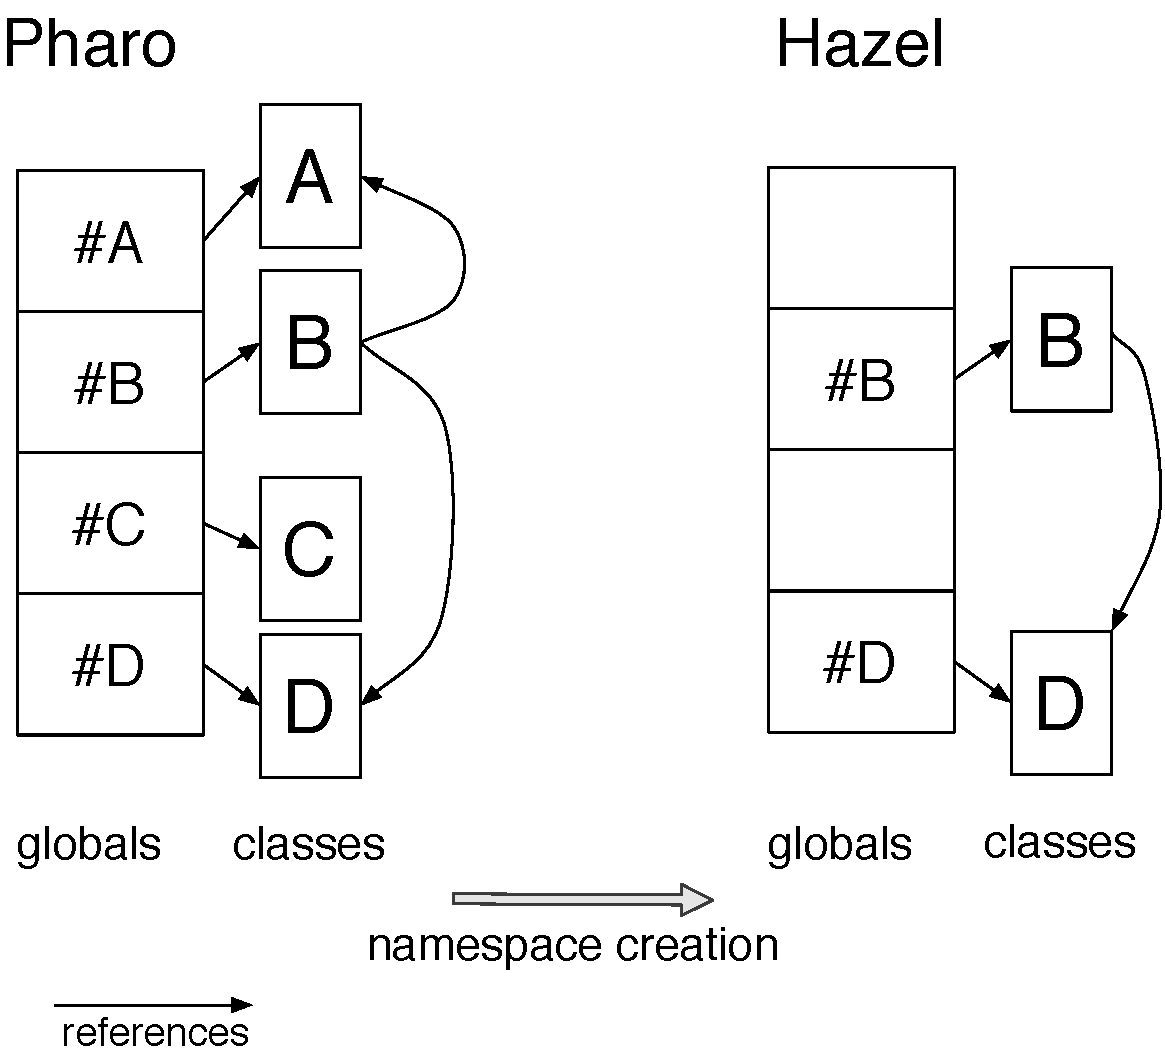
\includegraphics[height = 10cm]{figures/selfContainReference}
%	\caption{Kernel Isolated}
%	\label{KernelIsolated}
%\end{figure}


Now that the kernel is created, we need to isolate it by removing dependencies 
to the \gls{Pharo} world. There are two different types of dependencies which need to be fixed.

\subsection{References to unwanted classes}

\goal Here we want to remove dependencies from Hazel classes to \gls{Pharo} classes we haven't copied.

\problems
\begin{itemize}
	\item How to detect unwanted references ?
	\item How to remove those dependencies ?
	\item How to be sure it will not crash the system ?
\end{itemize}

\solutions
\begin{itemize}
	\item There are two places where unwanted references can be found:
		\begin{itemize}
			\item In a method: in a method literal there are references to invoke classes (see page~\pageref{literal}). Due to that, we can find references to unwanted classes;
			\item In a class variable\footnote{a class variable is a variable shared by all the instances of a class}: we can have an instance of an unwanted class or just an unwanted class itself.
		\end{itemize}
		The solution adopted is to check a class \ct{methodDictionary} and its class variables during class copy. If unwanted references are found, the following solution is applied.
	\item Removing dependencies is the key point of this cleaning step.
	
	For class variables, the solution was to set them to nil (in the minimal kernel creation process, only one class variable had to be set this way (\ct{HaloFont} from \ct{StandardFonts}).

		
	For methods we have considered several solutions. Our first thought was to remove the method and to recursively remove the sender of the method. But due to class structure,this would have removed almost all methods of the kernel. Then we thought about creating a \emph{NullPattern} object implementing all the removed methods. The problem was to find which kind of answer is expected from each method, and how to dynamically replace the sender in the code source. Finally we chose to remove the method and to keep the senders.
	\item We haven't found a solution to ensure that you are not creating an unstable system.
As long as your system can be changed, you can't certify that your kernel is totally functional.
We are working on a better isolation of the \gls{Pharo} kernel to reduce as much as possible the number of references (see Section~\ref{KernelFixes} page~\pageref{KernelFixes} ).
\end{itemize}

\inanutshell We have removed the references to unwanted class (see Figure~\ref{RemoveDependencies}), but because of that the integrity of the kernel may be corrupted.

%%NA: mettre la figure sous SVN
\begin{figure}[ht]
	\centering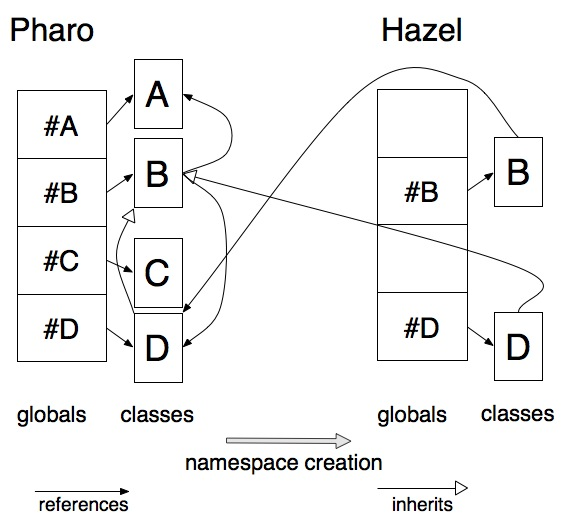
\includegraphics[width = 8cm]{figures/CleaningUnnecessaryRefWithInh}
	\caption{Step 2 - Remove references to unwanted classes}
	\label{RemoveDependencies}
\end{figure}

\newpage
\subsection{Dependencies from Hazel classes to original classes}

\goal Here we want to reroute dependencies from Hazel classes to \gls{Pharo} classes to have only intern references in the Hazel kernel. Those references are stored into methods literals.

\problems
\begin{itemize}
	\item How to change those references ?
	\item How to check what the kernel contains ?
\end{itemize}

\solutions 
\begin{itemize}
	\item This part is quite simple because the field was well prepared. Only methods refering copied classes are not fixed yet. So for those classes, the methodDictionary had just to be parsed in order to fix literals. And for fixing literals, we just change the \gls{Pharo} associations to their corresponding Hazel one (and we are sure it exists).
	\item To check what the new image actually contains, and to be able to modify it f needed, we have modified a bit a couple of tools to be able to browse the living kernel before its serialization.
\end{itemize}

\inanutshell We now have a kernel isolated with only internal references (see Figure~\ref{RerouteDependencies}).

\begin{figure}[ht]
	\centering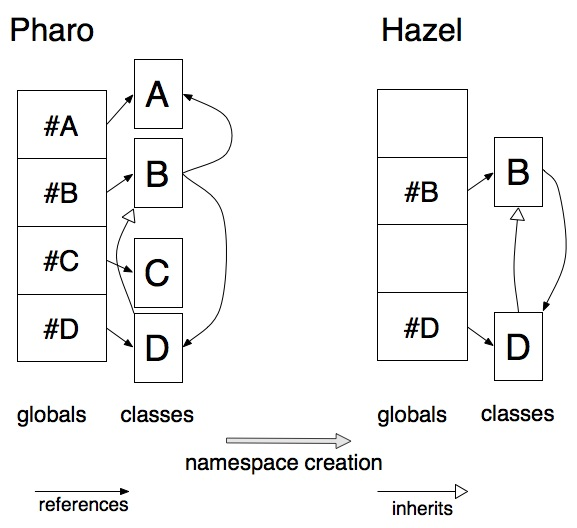
\includegraphics[width = 8cm]{figures/selfContainReferenceWIthInh}
	\caption{Step 3 - Reroute the remaining dependences}
	\label{RerouteDependencies}
\end{figure}









